\documentclass[12pt,a4paper]{article}
\usepackage{fullpage}
\pagestyle{plain}
% choose any of the following packages to support AmsTeX
%\usepackage{amsmath,amssymb,amsfonts,mathrsfs,mathptm,bm,mathtools}
% choose the following package to insert eps figures
% for png, jpg or pdf figures, use pdflatex
%\usepackage{graphicx}
\usepackage{amsmath}

%% Presenet code
\usepackage{listings}
\usepackage{color}
\usepackage{float}
\usepackage{graphicx}

\definecolor{dkgreen}{rgb}{0,0.6,0}
\definecolor{gray}{rgb}{0.5,0.5,0.5}
\definecolor{mauve}{rgb}{0.58,0,0.82}

\lstset{frame=tb,
  language=Python,
  aboveskip=3mm,
  belowskip=3mm,
  showstringspaces=false,
  columns=flexible,
  basicstyle={\small\ttfamily},
  numbers=none,
  numberstyle=\tiny\color{gray},
  commentstyle=\color{dkgreen},
  stringstyle=\color{mauve},
  breaklines=true,
  breakatwhitespace=true,
  tabsize=3
}



\newcommand{\question}[1]{\bigskip\noindent{\textbf{Q{#1} solution}}}

% set HW number
\newcommand{\HWnum}{5}
% specify first and last name and the ID number of students in the group
% append asterix to indicate who is making the submission
\newcommand{\StudentA}{Hanggang Zhu$^\ast$, 3200110457}
\newcommand{\StudentB}{Suhao Wang, 3200110777}
\newcommand{\StudentC}{Lumeng Xu 3200110184}

% ===============================================================
\begin{document}

%%% header
{\noindent \rule{\linewidth}{0.2mm}}\\
\noindent{ECE 374, ZJUI, Spring 2023\hfill%
  \textbf{\large H{}W\HWnum\ Solutions} \hfill \today\smallskip}

\noindent{\hfill \StudentA, \StudentB, and \StudentC \hfill}
\\[-0.2cm]{\noindent \rule{\linewidth}{0.2mm}}
%%% end header

% =============
\question{13.A}

In the naive Hanoi, disk n need to be moved from src to dest, with n - 1 disks in the tmp peg. But now it is forbidden to directly move disks move src to dest,the disk should be moved to tmp first and then moved to dest. So we need to move disks $n - 1$ to dest first (with intermediate begin on tmp peg), then move disk $n$ to tmp, move disks $n - 1$ from dest back to src(with intermediate being on tmp peg), move disk $n$ to dest and finally move disk $n -1 $ from src to dest again (with intermediate being on tmp peg). The correctness lies in that disk $n$ and disks $n - 1$ will be moved from src to dest, without violating rules.

The pseudo code is as follows:

\begin{lstlisting}
  Hanoi0(n, src, dest, tmp):
    if (n > 0) then
      Hanoi0(n - 1, src, dest, tmp)
      Move disk n from src to tmp
      Hanoi0(n - 1, dest, src, tmp)
      Move disk n from tmp to dest
      Hnaoi0(n - 1, src, dest, tmp)
\end{lstlisting}

The number of moves $T(n)$ can be represented as $T(n) = 3T(n - 1) + 2, n > 1$ with $T(1) = 2$. Solving the recurrence equation, we have $T(n) = 3^n - 1$

% =============

% =============
\question{13.B}\\
% =============
In this Hanoi 2, disk n need to be moved from src(peg1) to dest(peg2), with n - 1 disks in the tmp peg(peg0). But now it is forbidden to directly move disks move src to dest,the disk should be moved once at a time and it is not allowed to put a bigger disk on top of a smaller disk . So we need to move disks $n - 1$ to peg0 first with two steps, then move disk $n$ to dest(peg2), move disks $n - 1$ from dest back to src(peg1), and finally recursively move disk $n -1 $ from src(peg1) to dest(peg2) again . The correctness lies in that disk $n$ and disks $n - 1$ will be moved from src to dest, without violating rules.

The pseudo code is as follows:

\begin{lstlisting}
  Hanoi2(n, peg1, peg2, peg0):  //src,dest,tmp
    if (n > 0) then
      Hanoi2(n - 1, peg1, peg2, peg0)  	// n-1 in peg2
	   Hanoi2(n - 1, peg2, peg0, peg1)	  // n-1 in peg0
      Move disk n from peg1 to peg2
      Hanoi2(n - 1, peg0, peg1, peg2)		// n-1 in peg1
\end{lstlisting}

The number of moves $T(n)$ can be represented as $T(n) = 3T(n - 1) + 1, n > 1$ with $T(1) = 1$. Solving the recurrence equation, we have Upper bound $O(3^n)$


% =============
\question{13.C}

The largest remaining disk can be removed when nothing is on top of it. This is the same case in naive Hanoi when there's nothing on top largest remaining disk, we can move it to destination. So we can do modification to naive Hanoi with the difference that we remove the largest disk instead of moving it. The removed largest disk won't have any affect as in naive Hanoi the largest disk won't have any affect on rest of disks.

The pseudo code is as follows:
\begin{lstlisting}
  Hanoibyebye(n, src, dest, tmp, max_n):
    if (n > 0) then
      Hanoibyebye(n - 1, src, tmp, dest)
      if (n == max_n) then
        Remove disk n
      else
        Move disk n from src to tmp
      Hanoibyebye(n - 1, tmp, dest, src)
  
\end{lstlisting}

The number of moves $T(n)$ is the same as the case of naive Hanoi, where $T(n) = 2T(n - 1) + 1, n > 1$ with $T(1) = 1$. Solve the recurrence equation and there's $T(n) = 2^n - 1$. Upper bound is $O(2^n)$


% =============
\question{14.A}\\
% =============
$\bullet$ \textbf{The algorithm:}\\
We can use the array index of $A_1$,$A_2$,$\cdot \cdot \cdot$,$A_k$ as the basis for grouping. The problem of get the final big happy array now becomes getting two ordered arrays, Aleft and Aright, and then merge them.\\
Set $mid = left+\frac{right-left}{2}$. For the first division, $mid = 1+\frac{k-1}{2}$. Aleft contains all the element in the array $[A_1 \ \ to \ \ A_{mid}]$ and Aright will contains all the element in the array $[A_{mid}+1 \ \ to \ \ A_k]$.\\
Divide the big array recursively until there are only two arrays, then, skip the divide function and just merge them.\\
$\bullet$ \textbf{The time:}\\
There are k arrays at first, so the depth of the tree is at most $\log{k}$. In every layer, there are at most n times comparison. So $T(n) = O(nlogk)$.\\
$\bullet$ \textbf{the concept picture:} this is just an example.
	\begin{figure}[H]
	\centering %表示居中
	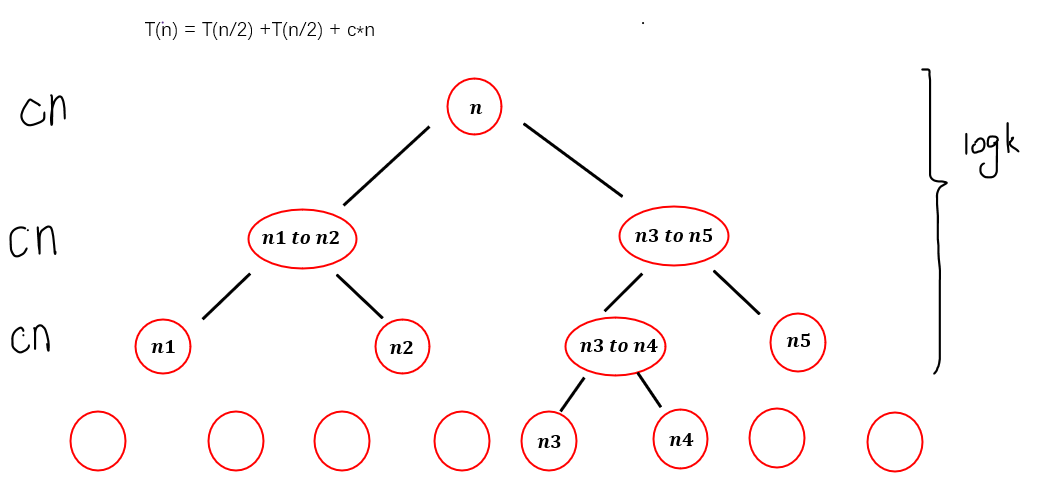
\includegraphics[height=5.5cm,width=12.5cm]{picture//Q14A.png}
	\caption{concept tree}
	\end{figure}
\noindent
$\bullet$ \textbf{Pseudocode:}\\
	left and right is the index of arrays from $A_1$ to $A_k$, result will store the final array, temp1,temp2 is used to store the children's sorted arrays.
	\begin{lstlisting}
	MergeSortA( left, right, result):
		if(right - left<1) then result = original array
		mid=left+(right-left)/2
		MergeSortA( left, mid, temp1)
		MergeSortA( mid+1, right, temp2)
		MergeTwo( temp1, temp2, result)


	MergeTwo ( t1, t2, result ):
		# use the pointer t1 and t2 to access the data
		i = 0, j= 0, k=0
		# len1 = the length of t1 array
		# len2 = the lenght of t2 array
		while ( i<=len1 and j<=len2 ):
			if ( t1 [ i ] <= t2[ j ] ):
				result [ k ] = t1[ i ]
				i=i+1
				k=k+1
			else:
				result [ k ] = t2[ i ]
				j=j+1
				k=k+1
	\end{lstlisting}


% =============
\question{14.B}\\
% =============
\textbf{If we are talking about merge sort with k-branch tree:}\\
$\bullet$ \textbf{The algorithm:}\\
Split the array of size N into k arrays with size $\frac{N}{k}$,\\
Now the question becomes sort the k arrays and merge them.\\
for every sub-arrays with size<>1, split them into k arrays with size $\frac{N}{k^2}$.\\. sort the new k arrays and merge them.\\
Do the recursive work and the final result is a big happy sorted array.\\
$\bullet$ \textbf{The time:}\\
The depth of the k-branches tree is $\log{k}$.\\
The comparision time of every layer is $cN$.\\
The running time is: $T(N) = kT(\frac{N}{k})+cN = O(NlogN)$\\	
$\bullet$ \textbf{the concept picture:}\\
	\begin{figure}[H]
	\centering %表示居中
	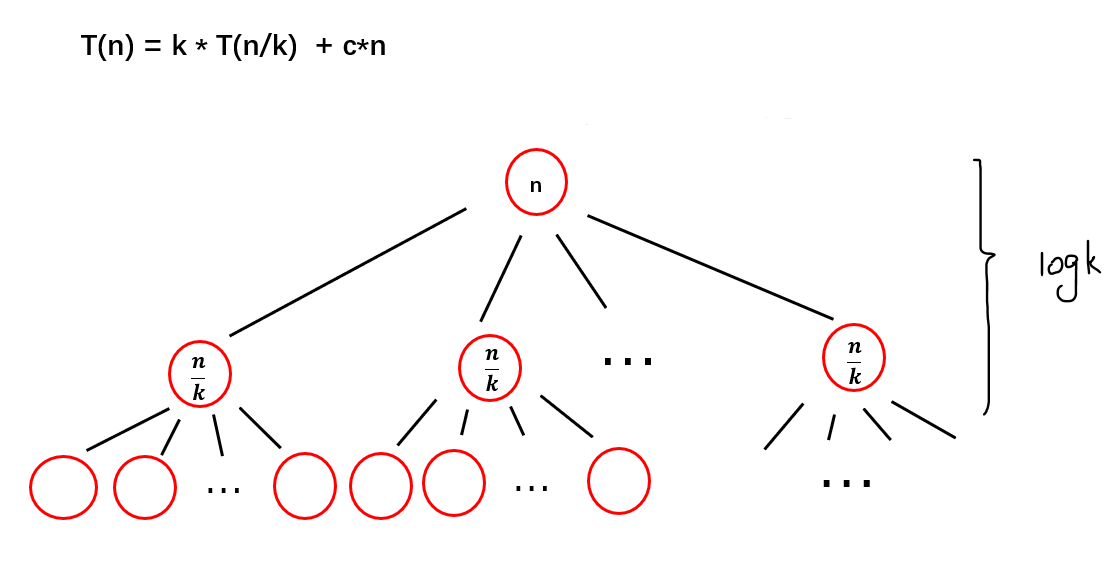
\includegraphics[height=5.5cm,width=12.5cm]{picture//Q14B1.png}
	\caption{concept tree}
	\end{figure}

\noindent
$\bullet$ \textbf{Pseudocode:}\\
	left and right is the index of arrays from $A_1$ to $A_n$, every array contains exactly one element at first. result will store the final array, t is the branch of the tree, temp is used to store the children's sorted arrays.
	\begin{lstlisting}
	MergeSortB( left, right, result, t):
		if(right - left<1) then result = original array
		count = 0
		while (count<t):
			mid [ i ] =left+(right-left)/t
			count= count+1
		
		count = 0
		while (count<t):
			temp [count] = MergeSortB( left, mid[count] , result, t )
			count= count+1
	
		Merge( temp, k, result )
	
	MergeB ( temp, t, result ):
		# merge data from temp[0] to temp [t-1] and stored into result
	\end{lstlisting}


\noindent
\textbf{If we are talking about Q14 with t-branch tree:}\\
$\bullet$ \textbf{The algorithm:}\\
Similar to the first question, suppose we use a t-branch tree for recursion.\\
Set (t-1) mid values.\\
We can use the array index of $A_1$,$A_2$,$\cdot \cdot \cdot$,$A_k$ as the basis for grouping. The problem of get the final big happy array now becomes getting k ordered arrays, $B_1$,$B_2$,$B_3$... and $B_k$, and then merge them.\\
Set $mid[i] = left+i \cdot \frac{right-left}{2}$. For the first division, $mid[i] = 1+i \cdot \frac{k-1}{2}$. $B_1$ contains all the element in the array $[A_1 \ \ to \ \ A_{mid[1]}]$ , for $i<k$, $B_i$ will contains all the element in the array $[A_{mid[i]}+1 \ \ to \ \ A_{mid[i+1]}]$.\\
Divide the big array recursively until there are only two arrays, then, skip the divide function and just merge them.\\
$\bullet$ \textbf{The time:}\\
The depth of the t-branches tree is $\log{k}$.\\
The comparision time of every layer is $cn$.\\
The running time is: $T(n) =  O(nlogk)$\\
$\bullet$ \textbf{the concept picture:} this is just an example.
	\begin{figure}[H]
	\centering %表示居中
	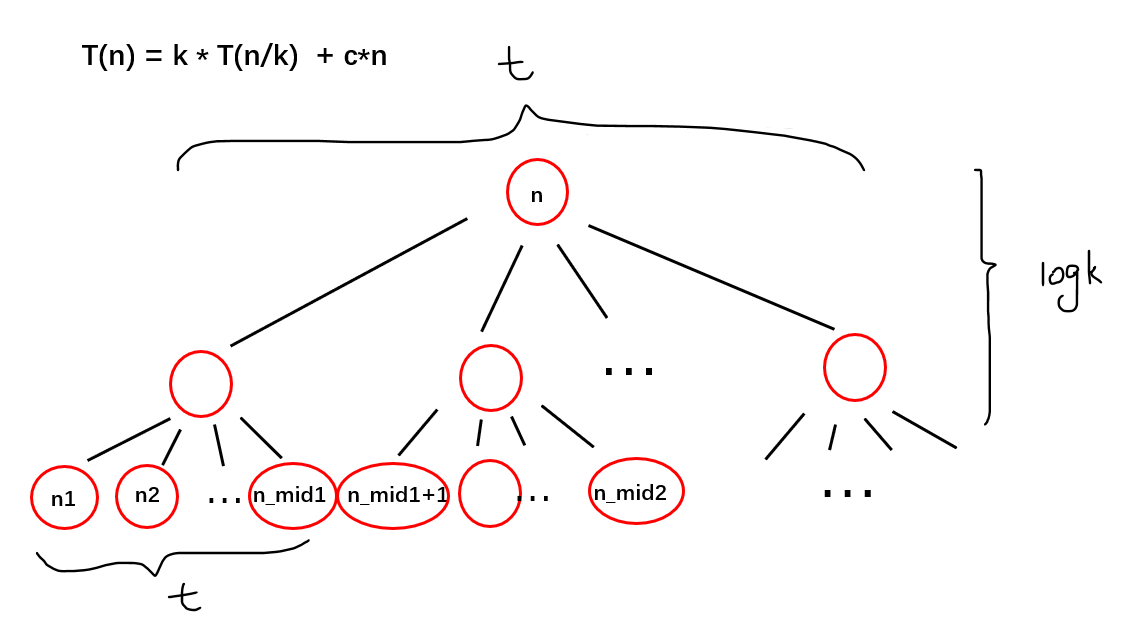
\includegraphics[height=5.5cm,width=12.5cm]{picture//Q14B2.png}
	\caption{concept tree}
	\end{figure}
\noindent
$\bullet$ \textbf{Pseudocode:}
	left and right is the index of arrays from $A_1$ to $A_k$, result will store the final array, t is the number of branch, temp is used to store the children's sorted arrays.
	\begin{lstlisting}
	MergeSortB( left, right, result, t):
		if(right - left<1) then result = original array
		count = 0
		while (count<t):
			mid [ i ] =left+(right-left)/t
			count= count+1
		
		count = 0
		while (count<t):
			temp [count] = MergeSortB( left, mid[count] , result, t )
			count= count+1
	
		Merge( temp, k, result )
	
	MergeB ( temp, t, result ):
		# merge data from temp[0] to temp [t-1] and stored into result
	\end{lstlisting}

% =============
\question{14.C}\\
% =============
$\bullet$ \textbf{The algorithm:}\\\\
Set an array $"temp"$ and $"result"$ to store the sorted array for each merge.\\
1. Traverse $k$ arrays in [$n_1$, $n_2$,.. ,$n_k$], find the one with the smallest $n_i$, record it in the array $temp$, and delete it from [$n_1$, $n_2$,.. ,$n_k$].\\
2. Traverse the $k-1$ array, find the one with the smallest $n_i$, merge it with $temp$, and store the result in the $result$. Overwrite the $temp$ array with $result$.\\
3. Traverse the $k-2$ array, find the one with the smallest $n_i$, merge it with $temp$, and store the result in the $result$. Overwrite the $temp$ array with $result$.\\\\
Cycle the above operations until [$n_1$, $n_2$,.. ,$n_k$] no longer has elements.\\
$\bullet$ \textbf{The time:}\\
the total Traverse time $T1 = k+k-1+k-2+...+1 = \frac{k+1}{2} = O(n)$\\
The depth of $n_i$ in the tree is $\log{\frac{n}{n_i}}$.\\
when merging $n_i$ to a higher layer, the merging time is $cn_i$.\\
The running time is: $T(n) = \frac{k+1}{2}+ \sum^k_{i=1}{n_i\log{\frac{n}{n_i}}} = O(n+\sum^k_{i=1}{n_i\log{\frac{n}{n_i}}})$\\
$\bullet$ \textbf{the concept picture:} assume that $n_1>n_2>n_3>$....$n_k$\\
	\begin{figure}[H]
	\centering %表示居中
	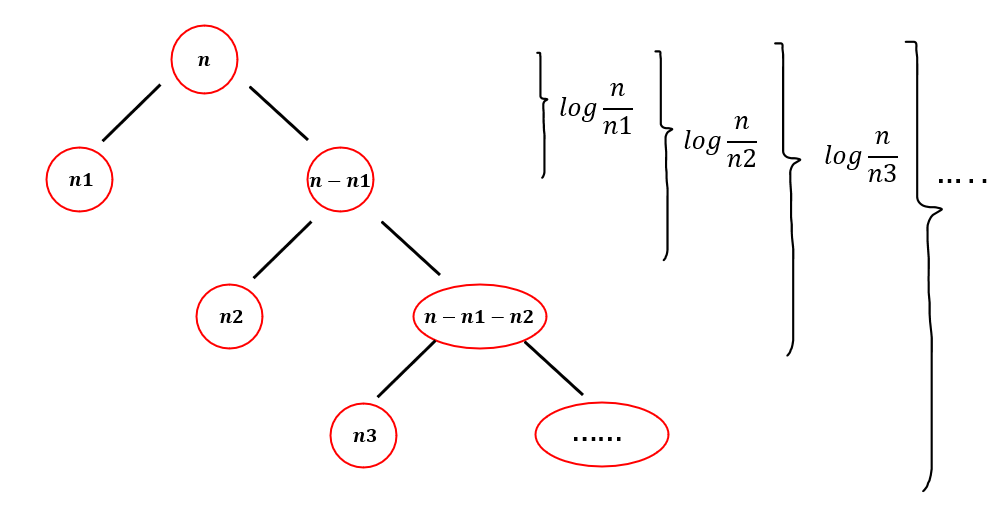
\includegraphics[height=5.5cm,width=12.5cm]{picture//Q14C2.png}
	\caption{concept tree}
	\end{figure}
\noindent
$\bullet$ \textbf{Pseudocode:}
	\begin{lstlisting}
	arr = [A1,A2,...,Ak]
	MergeSortC( arr, result, temp):
		# temp = the array pointer with the smallest ni found by Traverse
		# delete Ai in arr
		while (len(arr) <> 0 ):
			#  temp1 = the array pointer with the smallest ni found by Traverse
			# delete Ai in arr
			MergeTwo( temp1, temp , res)
			temp = res
			

	MergeTwo ( t1, t2, res ):
		# use the pointer t1 and t2 to access the data
		i = 0, j= 0, k=0
		# len1 = the length of t1 array
		# len2 = the lenght of t2 array
		while ( i<=len1 and j<=len2 ):
			if ( t1 [ i ] <= t2[ j ] ):
				result [ k ] = t1[ i ]
				i=i+1
				k=k+1
			else:
				result [ k ] = t1[ i ]
				j=j+1
				k=k+1
	\end{lstlisting}



\question{15.A}
\\We can use the Boyer-Moore Majority Vote Algorithm here. This algorithm works by maintaining a count of a candidate element that could be the majority element.
The count is incremented when an element is encountered that is equal to the candidate and decremented when it is not. If the count reaches zero, then a new candidate is chosen.
\\So, we can slove the problem according to the algorithm mentioned above:
\\The problem is finding the mode.
\\$\bullet$ \textbf{pairing period:}
\\(1) Set count=1.Choose $A$ bird a randomly, assuming that it is the mode, set $majority$=the original bird, and place it in a cage.
\\(2) Find another bird $B$ and put it in the cage, too.
\\(3) If they are friendly, remove $B$ from the cage, and then count=count+1
\\(4) If they are not friendly, remove $B$ from the cage and count=count-1
\\(5) Repeat operations 2, 3, and 4 above. If the number of count equals 0 during this process, move the original bird $A$ out of the cage, and then find a bird $C$ that has not been in the cage before. As the new mode $majority$, set count=1, and repeat 2, 3, and 4.
\\(6)"When all the birds have been caged, The $majority$ is the candidate species we are looking for. If there is a mode, then must be the "$majority$ species".
\\$\bullet$ \textbf{counting period:}
\\Traverse all the birds again to ensure that the "$majority$" is the mode.
\\$\bullet$ \textbf{identity period:}
\\Traverse all the birds again to  identifies every bird among the n birds that belong to this dominant species.
\\$\bullet$ \textbf{time analyze:}
\\ Since we just traverse the birds for several time, the time complexity of this algorithm is $O(n)$.
\\$\bullet$ \textbf{pseudo code:}
\\The pseudo code is as follows:
	\begin{lstlisting}
		FindMode(array, size):
	  		count=1
       	 	majority=array[0]
        		for i in range (1,size):
		            if(count==0): 
					majority=array[i]
		            if(array[i]==majority): 
					count=count+1
		            else: 
					count=count-1
			
			ensure = 0
        		for i in range (size):
		            if(array[i]==majority):
					 ensure = ensure+1
	  		if (ensure > size/2):
				return majority
	\end{lstlisting}


\question{15.B}
\\ For this question, because the number of species is determined to be $p$, we can use the method of counting votes to find out the plurality. It is not necessary to use Moore voting method.\\

\noindent
1. Maintain an array count [p] to count the number of each bird. Traverse n birds using a loop.\\

\noindent
2. Catch a bird $A_0$ and enter the $cage_0$, $count[0]= 1$\\

\noindent
3. Catch a bird $A_1$ into $cage_0$
\\ If $A_0$ and $A_1$ are friendly, then count [0]+1, move bird $A_1$
\\ If $A_0$ and $A_1$ are not friendly, place bird $A_1$ in $cage_1$, count [1]=1\\

\noindent
3. Catch a bird $A_2$ into $cage_j$, (j=0,1)
\\ If $A_j$ and $A_2$ are friendly, then count [j]+1, move bird $A_2$
\\ If $A_j$ and $A_2$ are not friendly, try next cage.
\\ When all cages are not friendly, place bird $A_2$ in $cage_2$, count [2]=1\\

\noindent
4. repeat until count[p-1]=1, Traverse the rest birds using a loop.\\


\noindent
5. Catch a bird $B$ into $cage_j$, (j=0,1,...,p)
\\ If $A_j$ and $B$ are friendly, then count [j]+1, move bird $B$
\\ If $A_j$ and $B$ are not friendly, try next cage.\\

\noindent
$\bullet$ \textbf{time analyze:}
\\ there are n birds, every birds have p comparisions. 
\\ $T(n) = cn \cdot p$
\\ The worst case is that the first p birds belong to different species [$cage_0$,$cage_1$,...$cage_{p-1}$], and the next (n-p) birds all belong to $cage_{p-1}$. It is smaller than $cn \cdot p$.
\\ So the time complexity is $O(n \cdot p)$

\end{document}
